\chapter{Eksperimen Sistem Permainan Musik Ekspresif untuk Alat Musik Gesek}

\section{Tujuan Eksperimen}

Eksperimen dilakukan untuk menunjukkan kinerja sistem permainan musik ekspresif untuk alat musik gesek yang telah dibangun. Sistem permainan musik ekspresif diimplementasi berdasarkan hasil perancangan pada Bab \ref{design-chapter}. Kinerja yang akan diukur adalah kealamian ekspresi hasil sintesis suara oleh sistem tersebut. Kealamian memiliki makna seberapa mirip ekspresi pada permainan yang dihasilkan terhadap ekspresi permainan manusia.

Meski tujuan utama eksperimen ini adalah menunjukkan kinerja sistem utuh, eksperimen juga dilakukan lebih detil untuk mengetahui kinerja komponen dan teknik yang digunakan. Secara ringkas, hal-hal yang diujikan tertulis dalam Tabel \ref{tab-experiment-list}.

Sebelum pengujian untuk menunjukkan kinerja sistem permainan musik ekspresif untuk alat musik gesek, dilakukan eksperimen penyetelan parameter untuk menentukan parameter-parameter terbaik. Hal ini karena arsitektur model dan pelatihannya dipengaruhi oleh berbagai parameter.

Selain itu, dilakukan juga pengujian untuk membuktikan bahwa skema pemilihan subset data latih yang diuraikan dalam Subbab \ref{subsetselectionsection} mampu menghasilkan model dengan kinerja lebih baik daripada model yang dilatih langsung menggunakan keseluruhan data latih untuk model-model yang menggunakan arsitektur Wavenet yang dimodifikasi. Hal ini akan dibuktikan untuk model-model \textit{pitch} dan \textit{timbre}. Adapun untuk model \textit{timing}, dilakukan pengujian untuk membuktikan bahwa skema pemilihan subset data latih tidak menghasilkan model dengan kinerja yang lebih baik daripada model yang dilatih langsung menggunakan keseluruhan data latih.

\begin{table}[htbp]
    \centering
    \caption{Tujuan Eksperimen yang Dilakukan}\label{tab-experiment-list}
    \begin{tabular}{ |p{0.2\textwidth}|p{0.325\textwidth}|p{0.325\textwidth}|p{0.15\textwidth}| }
    \hline
    &\textbf{Tujuan}&\textbf{Hipotesis}&\textbf{Metrik}\\\hline
    \multicolumn{4}{|p{\textwidth}|}{Eksperimen komponen}\\\hline
    Penyetelan parameter&Menentukan parameter terbaik&-&Koefisien korelasi\\\hline
    Uji pemilihan subset&Membuktikan hipotesis&
    - Model \text{pitch} dan \textit{timbre}: kinerja dengan pemilihan subset $>$ kinerja tanpa pemilihan subset&Koefisien korelasi \\
    && - model \text{textit}: kinerja dengan pemilihan subset $<$ kinerja tanpa pemilihan subset& \\hline
    Uji korelasi komponen&Mengetahui kinerja masing-masing komponen & - & koefisien korelasi \\\hline
    \multicolumn{4}{|p{\textwidth}|}{Eksperimen sistem utuh}\\\hline
    Uji korelasi sistem utuh&Membuktikan hipotesis & Kinerja teknik yang diajukan $>$ kinerja korelasi teknik \textit{baseline}& Koefisien korelasi\\\hline
    Uji preferensi kealamian&Membuktikan hipotesis & Pendengar manusia menganggap permainan dari sistem yang diajukan lebih alami daripada sistem \textit{baseline}& Preferensi kealamian subjektif \\\hline
    \end{tabular}
\end{table}

\section{Skenario Eksperimen}
Eksperimen dilakukan untuk menilai tingkat kealamian dari ekspresi permainan musik yang dihasilkan. Penilaian dilakukan dengan uji korelasi dan uji persepsi kealamian pendengar.

Eksperimen diawali dengan eksperimen komponen sistem untuk menyetel parameter dan menguji korelasi tiap-tiap model yang menjadi komponen dari sistem ini. Setelah itu, eksperimen dilakukan dengan eksperimen uji korelasi sistem utuh.

Pada eksperimen komponen, model-model \textit{timing}, \textit{pitch} yang terdiri dari model deviasi F0, dan \textit{timbre} yang terdiri dari model frekuensi harmonik, magnitudo harmonik, serta amplop stokastik disetel parameternya dan diuji korelasinya.

Untuk penyetelan parameter model-model, dilakukan validasi silang dengan $k=5$. Berikut ini adalah langkah-langkah validasi silang:
\begin{enumerate}
	\item data dibagi menjadi $k$ bagian
	\item untuk tiap bagian, gunakan bagian tersebut untuk memvalidasi model yang dilatih dengan komplemennya
	\item rata-ratakan metrik kinerja terhadap semua bagian tersebut
\end{enumerate}

Parameter-parameter model yang disetel berbeda-beda untuk tiap modelnya. Untuk model \textit{timing}, sebelum penyetelan parameter, dilakukan pemilihan teknik antara ANN dan regresi DT. Setelah itu, apabila teknik yang terpilih adalah DT, parameter yang disetel adalah jumlah not konteks yang menjadi fitur dan kedalaman maksimum.

Untuk model-model F0, frekuensi harmonik, magnitudo harmonik, dan amplop stokastik, terdapat empat kelompok parameter:
\begin{itemize}
	\item parameter-parameter yang diambil dari riset neural parametrik nyanyian, yaitu:
	\begin{itemize}
		\item ukuran konvolusi kausal awal
		\item ukuran kanal residual
		\item ukuran konvolusi terdilasi
		\item ukuran \textit{batch}
		\item jumlah \textit{frame} keluaran \textit{valid}
		\item \textit{learning rate} (awal, \textit{decay}, interval)
	\end{itemize}
	\item parameter-parameter yang bukan dari riset neural parametrik nyanyian, namun tidak disetel dengan validasi silang, yaitu:
	\begin{itemize}
		\item \textit{output stage}: tetap CGM, namun dimensi disesuaikan
		\item temperatur pembangkitan $\tau$: bilangan kecil, dimensi disesuaikan
		\item Jumlah \textit{epoch}: sedikit di atas jumlah epoch pada neural parametrik nyanyian, namun dibatasi dengan \textit{early stopping}
	\end{itemize}
	\item parameter yang disetel dengan validasi silang, yaitu:
	\begin{itemize}
		\item faktor dilasi
		\item tingkat \textit{noise} pada masukan $\lambda$
		\item \textit{early stopping patience}
	\end{itemize}
	\item parameter terikat, berubah apabila faktor dilasi dan ukuran konvolusi berubah, yaitu:
	\begin{itemize}
		\item jumlah lapisan
		\item jumlah lapisan per \textit{stage}
		\item medan reseptif
	\end{itemize}
\end{itemize}

Untuk model F0, parameter yang diambil dari riset neural parametrik nyanyian diambil dari model F0 pada riset neural parametrik nyanyian. Untuk model frekuensi harmonik dan model magnitudo harmonik, parameter disesuaikan dari model amplop harmonik pada riset neural parametrik nyanyian. Untuk model amplop stokastik, parameter disesuaikan dari model aperiodisitas pada riset neural parametrik nyanyian.

Setelah parameter telah disetel, model dilatih dengan keseluruhan data latih. Namun, model ini tidak langsung diujikan terhadap data uji. Kinerja model ini dibandingkan terlebih dahulu dengan kinerja model yang telah dilatih pada tahapan validasi silang. Hal ini dilakukan untuk memilih model terbaik, karena mungkin saja model yang dilatih dengan data latih lebih besar memiliki kinerja yang lebih buruk. Hal ini dilakukan untuk model \textit{pitch} dan model \textit{timbre}. Adapun untuk model \textit{timing} akan digunakan model yang dilatih dengan keseluruhan data latih. Setelah dipilih model yang terbaik terhadap data latih, model diujikan terhadap data uji.

Validasi, pengujian, dan pengukuran kinerja tiap-tiap model dilakukan sesuai dengan masukan dan keluaran model-model tersebut. Model \textit{timing} diberi masukan partitur dan divalidasi \textit{timing} hasilnya. Model F0 diberi masukan partitur dan \textit{timing} dan divalidasi F0 hasilnya. Demikian pula, serupa pada model frekuensi harmonik, magnitudo harmonik, hingga amplop stokastik.

Metrik yang digunakan adalah koefisien korelasi Pearson yang dituliskan pada persamaan \ref{pearson-corrcoef-eq}. Untuk model-model F0, frekuensi harmonik, magnitudo harmonik, dan amplop stokastik, koefisien korelasi dihitung pasangan nilai-nilai pada keluaran dan nilai-nilai pada data tiap \textit{frame}. Untuk model \textit{timing}, koefisien korelasi dihitung terhadap nilai nada, dalam skala nomor not midi, untuk tiap \textit{frame} berdasarkan \textit{timing} yang dihasilkan, berpasangan dengan nilai nada berdasarkan \textit{timing} data.

Model-model dengan parameter yang telah disetel dan dilatih dalam tahapan eksperimen komponen kemudian digabungkan untuk membentuk sistem utuh. Setelah itu, sistem utuh digunakan untuk membangkitkan suara dengan masukan partitur pada data uji. Keluaran akhirnya --sebelum diubah menjadi sinyal gelombang-- berupa frekuensi harmonik, magnitudo harmonik, serta amplop stokastik divalidasi dengan frekuensi harmonik, magnitudo harmonik, serta amplom stokastik pada data uji.

Pada bagian terakhir eksperimen, yaitu uji persepsi, dilakukan pengujian kepada sejumlah responden. Sebelum dilakukan uji pendengaran, ditanyakan kepada responden data pengalaman responden terkait musik. Pada uji pendengaran, responden diberikan 18 pasang segmen audio. Tiap pasang terdiri dari 10 detik segmen keluaran sistem yang telah dibangun dan 10 detik segmen keluaran sistem \textit{baseline}. Untuk tiap pasang, responden diminta untuk memilih segmen audio yang lebih alami. Dari hasil ini, dapat dihitung Mean Preference Score (MPS) sistem ini terhadap sistem \textit{baseline}.

Sistem yang dijadikan \textit{baseline} sebagai perbandingan adalah sistem Synful RPM. Untuk menghasilkan suara ekspresif, seharusnya sistem ini diberikan masukan partitur ekspresif. Namun, sebagai \textit{baseline} terhadap sistem yang dibangun, sistem ini diberi masukan yang sama dengan sistem yang telah dibangun yaitu partitur tanpa ekspresi.

\section{Hasil Eksperimen Komponen Sistem}

Hasil eksperimen komponen sistem terdiri dari eksperimen model \textit{timing}, \textit{pitch} yang terdiri dari model deviasi F0, dan \textit{timbre} yang terdiri dari model frekuensi harmonik, magnitudo harmonik, serta amplop stokastik. Eksperimen tiap-tiap model terdiri dari penyetelan parameter dan pengujian.

\subsection{Hasil penyetelan parameter}

Eksperimen model \textit{timing} dimulai dengan pemilihan teknik menggunakan validasi silang. Sebagaimana tampak pada Tabel \ref{tab-timing-model-tuning-results}, tampak bahwa teknik \textit{decision tree regression} memiliki kinerja yang lebih baik daripada ANN. Analisis lebih lanjut terhadap \textit{output} ANN tersebut menunjukkan bahwa deviasi \textit{timing} yang dihasilkan ANN adalah konstan. Hal ini menunjukkan bahwa ANN tidak dapat mempelajari pola deviasi \textit{timing} pada data latih.

\begin{table}[htbp]
    \centering
    \caption{Hasil Validasi Silang untuk Penyetelan Parameter Model \textit{Timing}}\label{tab-timing-model-tuning-results}
    \begin{tabular}{ |l|r| } 
     \hline
     Parameter & Pearson r untuk Nada Tiap \textit{Frame} \\
     \hline 
     \multicolumn{2}{|l|}{model regresi}\\ \hline
	 ann    &-0.03684115\\ \hline
	 dt, konteks=10, kedalaman=300     & 0.09796566\\ \hline
	 \multicolumn{2}{|l|}{penyetelan jumlah not konteks fitur}\\ \hline
	 dt, konteks=20, kedalaman=300       &0.07746795\\ \hline
	 dt, konteks=10, kedalaman=300      &0.09796566\\ \hline
	 dt, konteks=5, kedalaman=300     &0.14187831\\ \hline
	 dt, konteks=3, kedalaman=300     &\textbf{0.16475536}\\ \hline
	 dt, konteks=1, kedalaman=300      &0.10598458\\ \hline
	 \multicolumn{2}{|l|}{penyetelan kedalaman pohon}\\ \hline
	 dt, konteks=3, kedalaman=25 	 &0.15163629\\\hline
	 dt, konteks=3, kedalaman=50     &0.1326507\\\hline
	 dt, konteks=3, kedalaman=100      &0.12941929\\\hline
	 dt, konteks=3, kedalaman=300     &\textbf{0.16475536}\\ \hline
	 dt, konteks=3, kedalaman=600     &0.11958923\\\hline
	 dt, konteks=3, kedalaman=1000     &0.1351192   \\  \hline
    \end{tabular}
\end{table}

Hasil penyetelan parameter jumlah not konteks fitur dan kedalaman pohon juga terdapat pada Tabel \ref{tab-timing-model-tuning-results}. Parameter terbaik diperoleh dengan 3 not konteks fitur dan kedalaman pohon 300.

Penyetelan model berikutnya adalah penyetelan model F0. Tabel \ref{tab-f0-model-tuning-results} menunjukkan hasil validasi silang untuk penyetelan parameter model F0, dengan metrik berupa koefisien korelasi Pearson dari frekuensi fundamental hasil pembangkitan terhadap frekuensi fundamental pada data. Faktor dilasi yang menghasilkan kinerja terbaik adalah $1,2,4,8,16,32,1,2,4,8,16$. Faktor dilasi ini memiliki medan reseptif terhadap output sebelum yang lebih pendek daripada faktor dilasi pada riset neural parametrik nyanyian. Adapun tingkat \textit{noise} $\lambda$ terbaik didapatkan dengan nilai $0.4$, sama dengan pada riset neural parametrik nyanyian.

Pelatihan model F0 dengan \textit{early stopping} memiliki kinerja yang sama dengan pelatihan tanpa \textit{early stopping}. Hal ini karena dengan \textit{patience} 100, \textit{early stopping} tidak menghentikan pelatihan hingga jumlah \textit{epoch} maksimal yang bernilai 300. Karenanya, tanpa \textit{early stopping} ataupun dengan \textit{early stopping}, model F0 ini tetap dilatih dengan 300 \textit{epoch}.

\begin{table}[htbp]
    \centering
    \caption{Hasil Validasi Silang untuk Penyetelan Parameter Model F0}\label{tab-f0-model-tuning-results}
    \begin{tabular}{ |l|l|l|r| } 
     \hline
     \multicolumn{3}{|l|}{Parameter} & Pearson r\\
     \cline{1-3}
     faktor dilasi & $\lambda$ & \textit{patience} & F0\\
     \hline 
	1,2,4,8,16,32,64,1,2,4,8,16,32 & 0.4 &100      &0.9525\\\hline
	1,2,4,8,16,32,1,2,4,8,16 & 0.4 &100            &0.9526\\\hline
	1,2,4,8,16,32,64,1,2,4,8,16,32 & 0.01 &100     &0.9516\\\hline
	1,2,4,8,16,32,1,2,4,8,16 & 0.01 &100           &0.9507\\\hline
	1,2,4,8,16,32,1,2,4,8,16 & 0.4 &tanpa \textit{early stopping}    &0.9526\\\hline
    \end{tabular}
\end{table}

Hasil penyetelan parameter model frekuensi harmonik tampak pada Tabel \ref{tab-freq-model-tuning-results}. Faktor dilasi yang memiliki kinerja terbaik adalah $1,2,4,1,2$, sama dengan pada riset sintesis neural parametrik nyanyian. Tingkat \textit{noise} $\lambda$ terbaik adalah $0.4$, sama dengan pada riset sintesis neural parametrik nyanyian. Model yang dilatih dengan \textit{early stopping} memiliki kinerja lebih baik daripada tanpa \textit{early stopping}.

\begin{table}[htbp]
    \centering
    \caption{Hasil Validasi Silang untuk Penyetelan Parameter Model Frekuensi Harmonik}\label{tab-freq-model-tuning-results}
    \begin{tabular}{ |l|l|l|r| } 
     \hline
     \multicolumn{3}{|l|}{Parameter} & Rata-Rata Pearson r\\
     \cline{1-3}
     faktor dilasi & $\lambda$ & \textit{patience} &Frekuensi Harmonik \\
	 \hline 
	1,2,4,1,2 & 0.4 &100           &0.9888\\\hline
	1,2,4 & 0.4 &100               &0.9874\\\hline
	1,2,4,8,1,2,4 & 0.4 &100       &0.9884\\\hline
	1,2,4,1,2 & 0.01 &100          &0.9830\\\hline
	1,2,4 & 0.01 &100              &0.9884\\\hline
	1,2,4,8,1,2,4 & 0.01 &100      &0.9864\\\hline
	1,2,4,1,2 & 0.4 &tanpa \textit{early stopping}   &0.9839\\\hline
    \end{tabular}
\end{table}

Hasil penyetelan parameter model magnitudo harmonik tampak pada Tabel \ref{tab-mag-model-tuning-results}. Faktor dilasi yang memiliki kinerja terbaik adalah $1,2,4,8,1,2,4$. Faktor dilasi ini memiliki medan reseptif terhadap output sebelum yang lebih panjang daripada faktor dilasi pada riset neural parametrik nyanyian. Hal ini menunjukkan bahwa unsur magnitudo harmonik pada sintesis alat musik gesek membutuhkan konteks yang lebih luas daripada konteks pada sintesis suara nyanyian. Tingkat \textit{noise} $\lambda$ terbaik adalah $0.4$, sama dengan pada riset sintesis neural parametrik nyanyian. Model yang dilatih dengan \textit{early stopping} memiliki kinerja lebih baik daripada tanpa \textit{early stopping}.

\begin{table}[htbp]
    \centering
    \caption{Hasil Validasi Silang untuk Penyetelan Parameter Model Magnitudo Harmonik}\label{tab-mag-model-tuning-results}
    \begin{tabular}{ |l|l|l|r| } 
     \hline
     \multicolumn{3}{|l|}{Parameter} & Rata-Rata Pearson r\\
     \cline{1-3}
     faktor dilasi & $\lambda$ & \textit{patience} & Magnitudo Harmonik\\
	 \hline 
	1,2,4,1,2 & 0.4 &100           &0.1717\\\hline
	1,2,4,8,1,2,4 & 0.4 &100       &0.2002\\\hline
	1,2,4 & 0.4 &100               &0.0980\\\hline
	1,2,4,1,2 & 0.01 &100          &0.1338\\\hline
	1,2,4,8,1,2,4 & 0.01 &100      &0.0592\\\hline
	1,2,4 & 0.01 &100              &0.0556\\\hline
	1,2,4 & 0.4 &tanpa \textit{early stopping}       &0.1704\\\hline
    \end{tabular}
\end{table}

Hasil penyetelan parmeter model amplop stokastik tampak pada Tabel \ref{tab-stoc-model-tuning-results}. Faktor dilasi yang memiliki kinerja terbaik adalah $1,2,4,1,2$, sama dengan pada riset sintesis neural parametrik nyanyian. Tingkat \textit{noise} $\lambda$ terbaik adalah $0.4$, sama dengan pada riset sintesis neural parametrik nyanyian. Model yang dilatih dengan \textit{early stopping} memiliki kinerja lebih baik daripada tanpa \textit{early stopping}.

\begin{table}[htbp]
    \centering
    \caption{Hasil Validasi Silang untuk Penyetelan Parameter Model Amplop Stokastik}\label{tab-stoc-model-tuning-results}
    \begin{tabular}{ |l|l|l|r| } 
     \hline
     \multicolumn{3}{|l|}{Parameter} & Rata-Rata Pearson r\\
     \cline{1-3}
     faktor dilasi & $\lambda$ & \textit{patience} & Amplop Stokastik\\
	 \hline 
	1,2,4,1,2& 0.4& 100           & 0.0391\\\hline
	1,2,4& 0.4& 100               & 0.0729\\\hline
	1,2,4,8,1,2,4& 0.4& 100       &-0.0028\\\hline
	1,2,4,1,2& 0.01& 100          &-0.0328\\\hline
	1,2,4& 0.01& 100              &-0.0884\\\hline
	1,2,4,8,1,2,4& 0.01& 100      &-0.1304\\\hline
	1,2,4& 0.4& tanpa \textit{early stopping}       & 0.0493\\\hline
    \end{tabular}
\end{table}

Dengan demikian, nilai parameter-parameter model yang telah disetel terdapat pada Tabel \ref{tab-timbre-pitch-model-parameters} dan Tabel \ref{tab-timing-model-parameters}. Nilai parameter-parameter model \textit{timing} terdapat pada Tabel \ref{tab-timing-model-parameters}. Nilai parameter-parameter model \textit{pitch} dan model timbre terdapat pada Tabel \ref{tab-timbre-pitch-model-parameters}.
\begin{table}[htbp]
	\centering
	\caption{Nilai Parameter-Parameter Model \textit{Timing}}\label{tab-timing-model-parameters}
	\begin{tabular}{|l|l|}
	\hline
	Parameter&Nilai \\\hline
	Fitur not konteks & 3 sebelum, 3 sesudah\\\hline
	Kedalaman maksimal pohon & 300\\\hline
	\end{tabular}
\end{table}


\begin{table}[htbp]
	\newlength\colwidth
	\setlength\colwidth{\dimexpr.2\columnwidth-2\tabcolsep-0.2\arrayrulewidth\relax}
	\centering
	\caption{Nilai Parameter-Parameter Model \textit{Pitch} dan Model Timbre}\label{tab-timbre-pitch-model-parameters}
	\begin{tabular}{|p{\colwidth}|p{\colwidth}|p{\colwidth}|p{\colwidth}|p{\colwidth}|}
	\hline
	\multirow{2}{*}{Parameter}&\multicolumn{3}{|p{\dimexpr 3\colwidth}|}{Model Timbre}&{Model Pitch}\\\cline{2-5}
	&Deviasi Frekuensi Harmonik&Magnitudo Harmonik (ternormalisasi minmax)&Amplop Stokastik (ternormalisasi minmax)&Deviasi F0 (skala: \textit{semitone})\\\hline
	Dimensi fitur&20&20&6&1\\\hline
	Input tambahan (dim.)& Deviasi F0 (1) & Deviasi F0 (1) \newline Dev. HFreq (20) & Deviasi F0 (1) \newline Dev. HFreq (20) \newline Hmag (20) & - \\
	\hline
	Not konteks input kontrol & \multicolumn{4}{|p{\dimexpr 4\colwidth}|}{
	Not sebelum dan not sesudah
	}\\\hline
	Tingkat \textit{noise} $\lambda$ & 0.4&0.4&0.4&0.4\\\hline
	Temperatur pembangkitan & 0. (harmonik terendah) – 0.0001 (harmonik tertinggi) & 0. (harmonik terendah) – 0.01 (harmonik tertinggi) & 0.001 & 0.001 \\\hline
	Konvolusi kausal awal & $10 \times 1$ & $10 \times 1$ & $10 \times 1 $ & $20 \times 1 $\\\hline
	Kanal residual & 20 & 130 & 20 & 100 \\\hline
	Konvolusi terdilasi & $2\times 1$ & $2\times 1$ & $2\times 1$ & $2\times 1$ \\\hline
	Jumlah lapisan & 5 & 7 & 3 & 11\\\hline
	Lapisan per \textit{stage} & 3 & 4 & 3 & 6\\\hline
	Faktor dilasi & 1,2,4,1,2 & 1,2,4,8,1,2,4 & 1,2,4 & 1,2,4,8,16,32, 1,2,4,8,16\\\hline
	Medan reseptif&58 ms & 93 ms & 49 ms & 33 ms\\\hline
	Kanal \textit{skip}&16&240&20&100\\\hline
	\textit{Output stage}&Tanh$\rightarrow 1\times 1 \rightarrow 20\times CGM_{K=4}$&Tanh$\rightarrow 1\times 1 \rightarrow 20\times CGM_{K=4}$&Tanh$\rightarrow 1\times 1 \rightarrow 6\times CGM_{K=4}$&Tanh$\rightarrow 1\times 1 \rightarrow 1\times CGM_{K=4}$\\\hline
	Ukuran \textit{batch} &32&32&32& 64\\\hline
	Jumlah \textit{frame} output valid & 101 & 101 & 101 & 101 \\\hline
	\textit{Learning rate} & default & default & default & default\\\hline
	Jumlah \textit{epoch} maksimal & 2000 & 2000 & 2000 & 300 \\\hline
	\textit{Patience} & 100 & 100 & 100 & 100 \\\hline
	\end{tabular}
\end{table}
\subsection{Perbandingan kinerja model dari keseluruhan data latih dengan model dari sebagian data latih}

Tabel \ref{tab-timing-model-subset-results} menunjukkan perbandingan kinerja model \textit{timing} yang dilatih dengan keseluruhan data latih dan model yang dilatih dengan sebagian data latih. Hasil ini membuktikan bahwa untuk model \textit{timing}, model yang dilatih dengan keseluruhan data latih memiliki kinerja lebih baik. Adapun model yang dilatih dengan sebagian data latih, umumnya memiliki kinerja terhadap data uji yang lebih buruk. Hal ini karena model \textit{timing} tidak mengalami anomali yang dialami oleh model-model yang menggunakan arsitektur Wavenet yang dimodifikasi.

\begin{table}[htbp]
    \centering
    \caption{Kinerja Model Timing dengan Berbagai Subset Data Latih}\label{tab-timing-model-subset-results}
    \begin{tabular}{ |l|r|r| } 
     \hline
     \multirow{2}{*}{Subset data latih} & \multicolumn{2}{l|}{Pearson r untuk Nada Tiap \textit{Frame}} \\
     \cline{2-3}
     & terhadap data latih & terhadap data uji \\\hline

	\textit{fold}-1          &0.1816  &0.0528\\\hline
	\textit{fold}-2          &0.2049 &-0.0252\\\hline
	\textit{fold}-3          &0.2009  &0.1483\\\hline
	\textit{fold}-4          &0.2515  &0.0187\\\hline
	\textit{fold}-5          &0.2868  &0.0001\\\hline
	data latih utuh			 &0.2511  &0.2213\\\hline
    \end{tabular}
\end{table}

Tabel \ref{tab-f0-model-subset-results} menunjukkan perbandingan kinerja model F0 yang dilatih dengan keseluruhan data latih dan model yang dilatih dengan sebagian data latih. Perhatikan bahwa kinerja tertinggi terhadap data latih diperoleh dengan subset \textit{fold}-1. Kinerja model yang dilatih dengan subset ini terhadap data uji lebih baik daripada kinerja model yang dilatih dengan keseluruhan data latih. Hal ini menunjukkan bahwa untuk model F0, dengan memilih subset data latih dengan kinerja terhadap data latih tertinggi, kinerjanya kepada data uji lebih baik daripada model yang dilatih dengan data latih utuh. 

Terdapat dua kemungkinan yang menyebabkan hal ini. Kemungkinan pertama, penambahan data latih menurunkan kinerja. Kemungkinan kedua adalah kualitas data latih tidak merata.

\begin{table}[htbp]
    \centering
    \caption{Kinerja Model F0 dengan Berbagai Subset Data Latih}\label{tab-f0-model-subset-results}
    \begin{tabular}{ |l|r|r| } 
     \hline
     \multirow{2}{*}{Subset data latih} & \multicolumn{2}{l|}{Pearson r untuk F0 Tiap \textit{Frame}} \\
     \cline{2-3}
     & terhadap data latih & terhadap data uji \\\hline
	\textit{fold}-1          &0.9529  & 0.9551\\\hline
	\textit{fold}-2          &0.9511  &-0.9534\\\hline
	\textit{fold}-3          &0.9520  &0.9534\\\hline
	\textit{fold}-4          &0.9512  &0.9547\\\hline
	\textit{fold}-5          &0.9513  &0.9547\\\hline
	data latih utuh			 &0.9514  &0.9547\\\hline
    \end{tabular}
\end{table}

Tabel \ref{tab-freq-model-subset-results} menunjukkan  perbandingan kinerja model frekuensi harmonik yang dilatih dengan keseluruhan data latih dan model yang dilatih dengan sebagian data latih. Perhatikan bahwa kinerja tertinggi terhadap data latih diperoleh dengan data latih utuh. Kinerja tertinggi terhadap data uji juga didapatkan dengan model yang dilatih dengan data latih utuh. 

Hal ini menunjukkan bahwa untuk model frekuensi harmonik, penambahan data latih meningkatkan kinerja model. Selain itu, ditunjukkan pula bahwa untuk model frekuensi harmonik, pemilihan kumpulan data latih berdasarkan kinera terhadap data latih utuh akan menghasilkan kinerja tertinggi terhadap data uji.

\begin{table}[htbp]
    \centering
    \caption{Kinerja Model Frekuensi Harmonik dengan Berbagai Subset Data Latih}\label{tab-freq-model-subset-results}
    \begin{tabular}{ |l|r|r| } 
     \hline
     \multirow{2}{*}{Subset data latih} & \multicolumn{2}{l|}{Pearson r untuk Frekuensi Harmonik Tiap \textit{Frame}} \\
     \cline{2-3}
     & terhadap data latih & terhadap data uji \\\hline
	\textit{fold}-1      &0.9897  &0.9924\\\hline
	\textit{fold}-2      &0.9898  &0.9917\\\hline
	\textit{fold}-3      &0.9909  &0.9924\\\hline
	\textit{fold}-4      &0.9868  &0.9930\\\hline
	\textit{fold}-5      &0.9896  &0.9932\\\hline
	data latih utuh      &0.9920  &0.9935\\\hline
    \end{tabular}
\end{table}

Tabel \ref{tab-mag-model-subset-results} menunjukkan perbandingan kinerja model magnitudo harmonik yang dilatih dengan keseluruhan data latih dan model yang dilatih dengan sebagian data latih. Perhatikan bahwa kinerja tertinggi terhadap data latih diperoleh dengan subset \textit{fold}-5. Kinerja model yang dilatih dengan subset ini terhadap data uji lebih baik daripada kinerja model yang dilatih dengan keseluruhan data latih. Hal ini menunjukkan bahwa untuk model magnitudo harmonik, dengan memilih subset data latih dengan kinerja terhadap data latih tertinggi, kinerjanya kepada data uji lebih baik daripada model yang dilatih dengan data latih utuh. 

Perhatikan pula bahwa kinerja model yang dilatih dengan subset \textit{fold}-1 hingga \textit{fold}-5 memiliki kinerja terhadap data latih utuh yang lebih tinggi dibandingkan dengan model yang dilatih dengan data latih utuh. Begitu pula kinerja terhadap data uji dari model yang dilatih dengan subset \textit{fold}-1 hingga \textit{fold}-5 secara umum lebih baik daripada model yang dilatih dengan data latih utuh. Hal ini menunjukkan bahwa untuk model magnitudo harmonik, data latih yang berukuran lebih besar memiliki kinerja lebih rendah.

\begin{table}[htbp]
    \centering
    \caption{Kinerja Model Magnitudo Harmonik dengan Berbagai Subset Data Latih}\label{tab-mag-model-subset-results}
    \begin{tabular}{ |l|r|r| } 
     \hline
     \multirow{2}{*}{Subset data latih} & \multicolumn{2}{l|}{Pearson r untuk Magnitudo Harmonik Tiap \textit{Frame}} \\
     \cline{2-3}
     & terhadap data latih & terhadap data uji \\\hline
	\textit{fold}-1      &0.3997  &0.3031\\\hline
	\textit{fold}-2      &0.3846  &0.2725\\\hline
	\textit{fold}-3      &0.4118  &0.2469\\\hline
	\textit{fold}-4      &0.3886  &0.2972\\\hline
	\textit{fold}-5      &0.4469  &0.3211\\\hline
	data latih utuh    	 &0.3050  &0.2534\\\hline
    \end{tabular}
\end{table}

\begin{figure}[htbp]
    \centering
    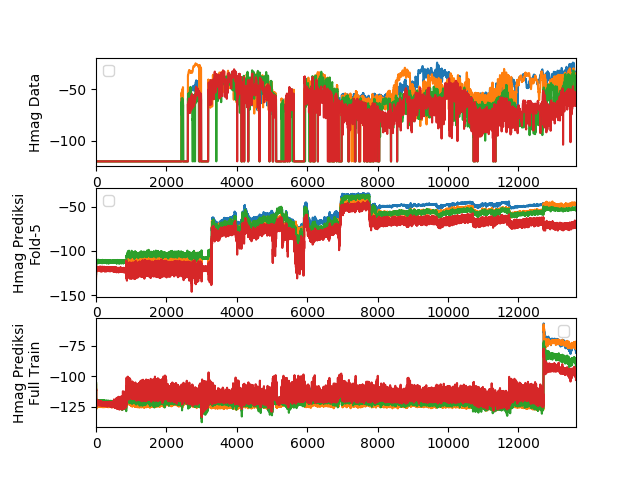
\includegraphics[width=0.8\textwidth]{resources/Analisis_Hmag_subset.png}
    \caption{Contoh Perbandingan Keluaran Model Magnitudo Harmonik yang Dilatih dengan Subset dan Keseluruhan Data Latih (4 Harmonik Pertama), dengan Masukan \textit{Timing}, F0, dan Hfreq dari Dataset}\label{fig-hmag-subset-output-sample}
\end{figure}

Gambar \ref{fig-hmag-subset-output-sample} menujukkan contoh perbandingan keluaran model magnitudo harmonik yang dilatih dengan subset dan yang dilatih dengan keseluruhan data latih. Grafik paling atas menunjukkan referensi pada data, grafik tengah menunjukkan keluaran dari model yang dilatih dengan subset \textit{fold}-5, dan grafik paling bawah menunjukkan keluaran dari model yang dilatih dengan keseluruhan data latih. Tampak bahwa model yang dilatih dengan keseluruhan data latih lebih banyak menghasilkan magnitudo kecil. Pada taraf magnitudo -100 hingga -120 dB seperti pada gambar tersebut, pendengar akan mendengar seolah-olah tidak ada suara.

Tabel \ref{tab-stoc-model-subset-results} menunjukkan perbandingan kinerja model stokastik yang dilatih dengan keseluruhan data latih dan model yang dilatih dengan sebagian data latih. Perhatikan bahwa kinerja tertinggi terhadap data latih diperoleh dengan subset \textit{fold}-1. Kinerja model yang dilatih dengan subset ini terhadap data uji lebih baik daripada kinerja model yang dilatih dengan keseluruhan data latih. Hal ini menunjukkan bahwa untuk model stokastik, dengan memilih subset data latih dengan kinerja terhadap data latih tertinggi, kinerjanya kepada data uji lebih baik daripada model yang dilatih dengan data latih utuh. 

Terdapat dua kemungkinan yang menyebabkan hal ini. Kemungkinan pertama, penambahan data latih menurunkan kinerja. Kemungkinan kedua adalah kualitas data latih tidak merata.

\begin{table}[htbp]
    \centering
    \caption{Kinerja Model Amplop Stokastik dengan Berbagai Subset Data Latih}\label{tab-stoc-model-subset-results}
    \begin{tabular}{ |l|r|r| } 
     \hline
     \multirow{2}{*}{Subset data latih} & \multicolumn{2}{l|}{Pearson r untuk Amplop Stokastik Tiap \textit{Frame}} \\
     \cline{2-3}
     & terhadap data latih & terhadap data uji \\\hline
	\textit{fold}-1       &0.2471  &0.0211\\\hline
	\textit{fold}-2       &0.5555  &0.0508\\\hline
	\textit{fold}-3       &0.2820  &0.0355\\\hline
	\textit{fold}-4       &0.5925  &0.0640\\\hline
	\textit{fold}-5       &0.5598  &0.1240\\\hline
	data latih utuh       &0.4303  &0.0552\\\hline
    \end{tabular}
\end{table}

Dengan demikian, dapat diambil kesimpulan untuk skema pemilihan subset. Untuk model \textit{timing}, kinerja model yang dilatih dengan keseluruhan dataset lebih besar daripada model yang dilatih dengan subset yang dipilih dengan skema tersebut. Untuk model frekuensi harmonik, dari skema pemilihan tersebut dipilih data latih utuh, sehingga kinerja dengan skema tersebut sama dengan apabila model dilatih tanpa skema pemilihan subset data latih. Untuk model F0, magnitudo harmonik, dan amplop stokastik, model yang dilatih dengan dataset yang dipilih dengan skema pemilihan subset menghasilkan kinerja yang lebih baik daripada model yang dilatih dengan data latih utuh.

Dengan demikian, pernyataan pada riset neural parametrik nyanyian bahwa penambahan data latih dapat menurunkan kinerja. Untuk jaringan syaraf tiruan dengan arsitektur Wavenet yang dimodifikasi, penambahan data latih dapat menurunkan kinerja. Adapun untuk model \textit{timing} yang tidak menggunakan arsitektur tersebut, penambahan data latih tetap meningkatkan kinerja.

\subsection{Hasil Uji Korelasi Tiap Komponen}

Tabel \ref{tab-timing-testing-results} menunjukkan korelasi nada tiap-tiap \textit{frame} dengan \textit{timing} not keluaran model \textit{timing}. Korelasi ini diukur terhadap nada tiap-tiap \textit{frame} dengan \textit{timing} ekspresif pada data. Nilai koefisien korelasi di atas 0 menunjukkan bahwa model berhasil mempelajari pola \textit{timing}. Namun, koefisien korelasi ini masih bernilai rendah. Kinerja model ini rendah baik terhadap data latih maupun data uji. Hal ini menunjukkan adanya \textit{underfitting}.

\begin{table}[htbp]
    \centering
    \caption{Hasil Uji Korelasi Model Timing}\label{tab-timing-testing-results}
    \begin{tabular}{ |l|r|r| } 
     \cline{2-3}
     \multicolumn{1}{l|}{}&Terhadap data latih&Terhadap data uji\\\hline
	 Pearson r&0.2511  &0.2213\\\hline
    \end{tabular}
\end{table}
%TODO analisis hasil eksperimen model timing

Tabel \ref{tab-f0-testing-results} menunjukkan koefisien korelasi f0 tiap-tiap \textit{frame} keluaran model f0 terhadap f0 pada data. Nilai koefisien korelasi di atas 0 menunjukkan bahwa model berhasil mempelajari pola f0. Koefisien korelasi model ini tidak mencapai nilai 1, namun sudah mencapai 0.9550 terhadap data uji. Tidak terjadi \textit{overfitting} di sini.
\begin{table}[htbp]
    \centering
    \caption{Hasil Uji Korelasi Model F0}\label{tab-f0-testing-results}
    \begin{tabular}{ |l|r|r| } 
     \cline{2-3}
     \multicolumn{1}{l|}{}&Terhadap data latih&Terhadap data uji\\\hline
	 Pearson r&0.9529  &0.9550\\\hline
    \end{tabular}
\end{table}

\begin{figure}[h]
    \centering
    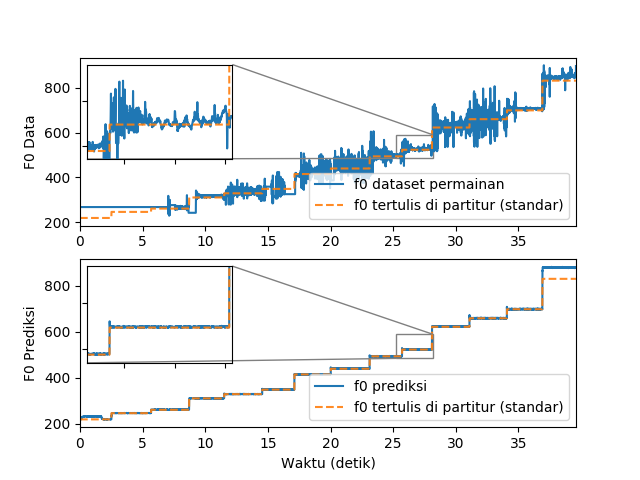
\includegraphics[width=0.8\textwidth]{resources/Analisis_F0.png}
    \caption{Contoh Keluaran Model F0, dengan Masukan \textit{Timing} dari Dataset}\label{fig-f0-output-sample}
\end{figure}

Kekurangan yang masih terjadi di model F0 adalah menganggap perubahan jangka-pendek dari F0 sebagai \textit{noise} dan hanya dirata-ratakan oleh model. Hal ini tampak pada contoh keluaran model F0 pada Gambar \ref{fig-f0-output-sample}. Pada bagian atas terlihat contoh F0 dari dataset, sedangkan pada bagian bawah terlihat F0 prediksi untuk sampel tersebut. Pada kedua bagian tersebut, terdapat bagian yang diperbesar untuk melihat perubahan jangka-pendek F0 tersebut. 

Pada bagian yang diperbesar pada gambar tersebut, terlihat dua jenis perubahan jangka-pendek F0 yang dianggap sebagai \textit{noise} oleh model. Pada bagian kiri, terlihat \textit{spike} pada data dianggap sebagai \textit{noise} oleh model, dan pada F0 prediksi hal tersebut hilang. Pada bagian kanan dari perbesaran tersebut pada F0 dari data, terlihat pola osilasi yang menunukkan \textit{vibrato}. Pada F0 prediksi hal tersebut hilang dan dirata-ratakan.

Tabel \ref{tab-freq-testing-results} menunjukkan koefisien korelasi frekuensi harmonik tiap-tiap \textit{frame} keluaran model frekuensi harmonik terhadap frekuensi harmonik pada data. Nilai koefisien korelasi di atas 0 menunjukkan bahwa model berhasil mempelajari pola frekuensi harmonik. Koefisien korelasi model ini tidak mencapai nilai 1, namun sudah mencapai 0.9550 terhadap data uji. Tidak terjadi \textit{overfitting} di sini.
\begin{table}[htbp]
    \centering
    \caption{Hasil Uji Korelasi Model Frekuensi Harmonik}\label{tab-freq-testing-results}
    \begin{tabular}{ |l|r|r| } 
     \cline{2-3}
     \multicolumn{1}{l|}{}&Terhadap data latih&Terhadap data uji\\\hline
	 Pearson r&0.9920  &0.9935\\\hline
    \end{tabular}
\end{table}

\begin{figure}[h]
    \centering
    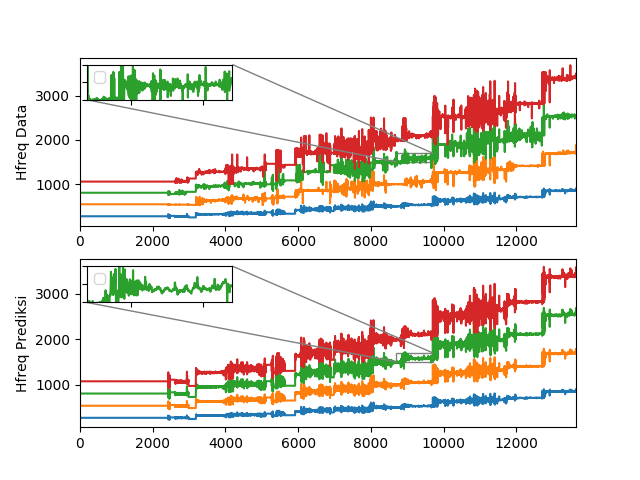
\includegraphics[width=0.8\textwidth]{resources/Analisis_Hfreq.png}
    \caption{Contoh Keluaran Model Frekuensi Harmonik (4 Harmonik Pertama), dengan Masukan \textit{Timing} dan F0 dari Dataset}\label{fig-hfreq-output-sample}
\end{figure}

Kekurangan yang masih terjadi di model frekuensi harmonik adalah menganggap perubahan jangka-pendek dari frekuensi harmonik sebagai \textit{noise} dan hanya dirata-ratakan oleh model. Hal ini tampak pada contoh keluaran model frekuensi harmonik pada Gambar \ref{fig-hfreq-output-sample}. Pada bagian atas terlihat contoh frekuensi harmonik dari dataset, sedangkan pada bagian bawah terlihat frekuensi harmonik prediksi untuk sampel tersebut. Pada kedua bagian tersebut, terdapat bagian yang diperbesar untuk melihat perubahan jangka-pendek frekuensi harmonik tersebut. 

Pada bagian yang diperbesar pada gambar tersebut, terlihat bahwa pola \textit{spike} dari deviasi frekuensi harmonik hilang, dan hanya dirata-ratakan saja. Padahal, pada dataset, untuk harmonik tinggi, terdapat pola seperti \textit{spike}. Adapun \textit{vibrato} dari F0 diteruskan ke harmonik selanjutnya, tanpa deviasi.

Tabel \ref{tab-mag-testing-results} menunjukkan koefisien korelasi magnitudo harmonik tiap-tiap \textit{frame} keluaran model magnitudo harmonik terhadap magnitudo harmonik pada data. Nilai koefisien korelasi di atas 0 menunjukkan bahwa model berhasil mempelajari pola magnitudo harmonik. Namun, koefisien korelasi ini masih bernilai rendah. Kinerja model ini rendah baik terhadap data latih maupun data uji. Hal ini menunjukkan adanya \textit{underfitting}.

\begin{table}[htbp]
    \centering
    \caption{Hasil Uji Korelasi Model Magnitudo Harmonik}\label{tab-mag-testing-results}
    \begin{tabular}{ |l|r|r| } 
     \cline{2-3}
     \multicolumn{1}{l|}{}&Terhadap data latih&Terhadap data uji\\\hline
	 Pearson r&0.4469  &0.3211\\\hline
    \end{tabular}
\end{table}

\begin{figure}[htbp]
    \centering
    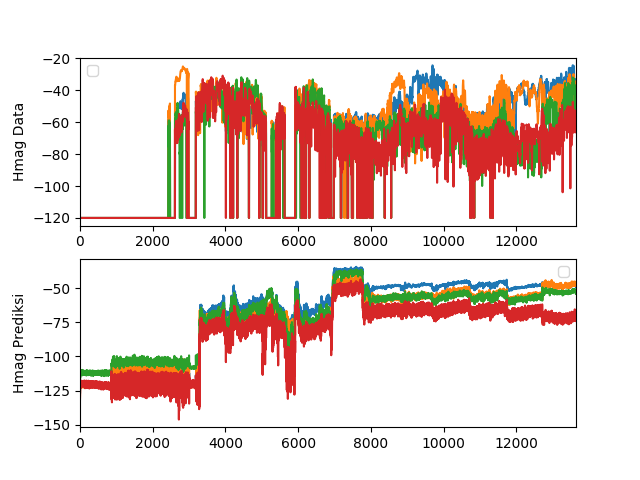
\includegraphics[width=0.8\textwidth]{resources/Analisis_Hmag.png}
    \caption{Contoh Keluaran Model Magnitudo Harmonik (4 Harmonik Pertama), dengan Masukan \textit{Timing}, F0, dan Hfreq dari Dataset}\label{fig-hmag-output-sample}
\end{figure}

\begin{figure}[htbp]
    \centering
    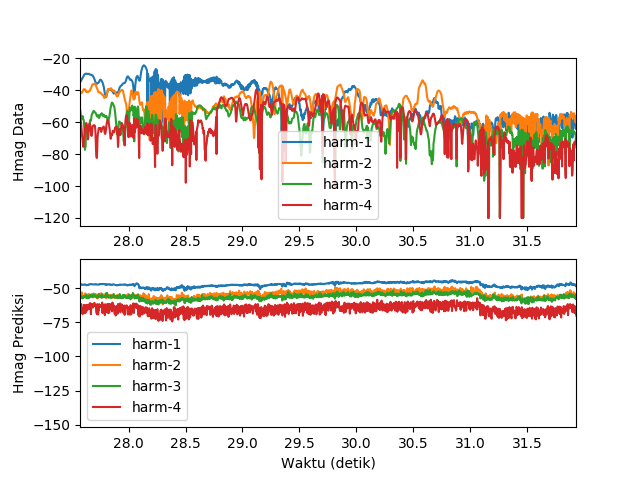
\includegraphics[width=0.8\textwidth]{resources/Analisis_Hmag_zoomed.png}
    \caption{(Diperbesar ke Satu Not) Contoh Keluaran Model Magnitudo Harmonik (4 Harmonik Pertama), dengan Masukan \textit{Timing}, F0, dan Hfreq dari Dataset}\label{fig-hmag-output-sample-zoomed}
\end{figure}

Kekurangan yang masih terjadi di model magnitudo harmonik adalah menganggap perubahan jangka-pendek dari magnitudo harmonik sebagai \textit{noise} dan hanya dirata-ratakan oleh model. Hal ini tampak pada contoh keluaran model magnitudo harmonik pada Gambar \ref{fig-hmag-output-sample}. Pada bagian atas terlihat contoh magnitudo harmonik dari dataset, sedangkan pada bagian bawah terlihat magnitudo harmonik prediksi untuk sampel tersebut. Tampilan yang diperbesar tampak pada gambar \ref{fig-hmag-output-sample-zoomed}.

Tampak bahwa model ini mampu membangkitkan ekspresi naik turunnya magnitudo secara umum. Namun, pola jangka-pendek yang dihasilkan berbeda dengan dataset. Terdapat beberapa perbedaan antara magnitudo harmonik pada dataset dan magnitudo harmonik yang dibangkitkan dengan model:

\begin{itemize}
	\item magnitudo harmonik pada dataset saling menyeberangi satu sama lain, sedangkan magnitudo harmonik bangkitan berurutan
	\item magnitudo harmonik pada dataset memiliki pola \textit{spike} yang jarang namun besar, sedangkan magnitudo harmonik bangkitan memiliki \textit{noise} yang kecil namun ada di semua tempat
	\item magnitudo harmonik pada dataset memiliki bukit-bukit/punuk-punuk sedangkan magnitudo harmonik bangkitan tidak memilikinya
	\item magnitudo harmonik pada dataset memiliki bentuk yang berbeda pada transisi not, sedangkan magnitudo harmonik bangkitan memiliki bentuk yang serupa sepanjang not
\end{itemize}

Perbedaan-perbedaan ini terjadi karena model tidak cukup kompleks untuk menangkap pola detil jangka-pendek dari magnitudo harmonik dataset. Alih-alih mendapatkan pola magnitudo harmonik yang saling menyeberangi satu sama lain, model hanya menangkap pola umum rata-rata rasio magnitudo antar harmonik. Bentuk bukit-bukit/punuk-punuk dan \textit{spike} yang jarang ditangkap sebagai \textit{noise} yang direpresentasikan dengan nilai variansi pada keluaran CGM.

Model ini juga tidak mampu memisahkan antara transisi not, awal not, akhir not, dan pertengahan not dari sisi bentuk. Ia hanya mampu mempelajari pola naik turun magnitudo secara umum. Pada hasil uji persepsi kealamian, akan tampak apakah perbedaan bentuk ini mempengaruhi persepsi kealamian.

Tabel \ref{tab-stoc-testing-results} menunjukkan koefisien korelasi amplop stokastik tiap-tiap \textit{frame} keluaran model amplop stokastik terhadap amplop stokastik pada data. Nilai koefisien korelasi di atas 0 menunjukkan bahwa model berhasil mempelajari pola amplop stokastik. Namun, koefisien korelasi ini masih bernilai rendah. Kinerja model ini rendah baik terhadap data latih maupun data uji. Namun, kinerja terhadap data uji jauh lebih rendah daripada kinerja terhadap data latih. Hal ini menunjukkan bahwa baik galat pelatihan maupun galat generalisasi pada model ini masih sangat tinggi.

\begin{table}[htbp]
    \centering
    \caption{Hasil Uji Korelasi Model Amplop Stokastik}\label{tab-stoc-testing-results}
    \begin{tabular}{ |l|r|r| } 
     \cline{2-3}
     \multicolumn{1}{l|}{}&Terhadap data latih&Terhadap data uji\\\hline
	 Pearson r&0.5925  &0.0640\\\hline
    \end{tabular}
\end{table}

\begin{figure}[htbp]
    \centering
    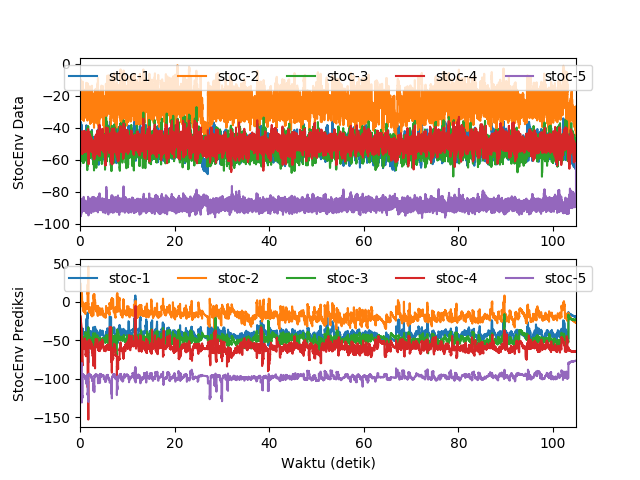
\includegraphics[width=0.8\textwidth]{resources/Analisis_StocEnv.png}
    \caption{Contoh Keluaran Model Amplop Stokastik, dengan Masukan \textit{Timing}, F0, dan Hfreq dari Dataset}\label{fig-stocenv-output-sample}
\end{figure}

\begin{figure}[htbp]
    \centering
    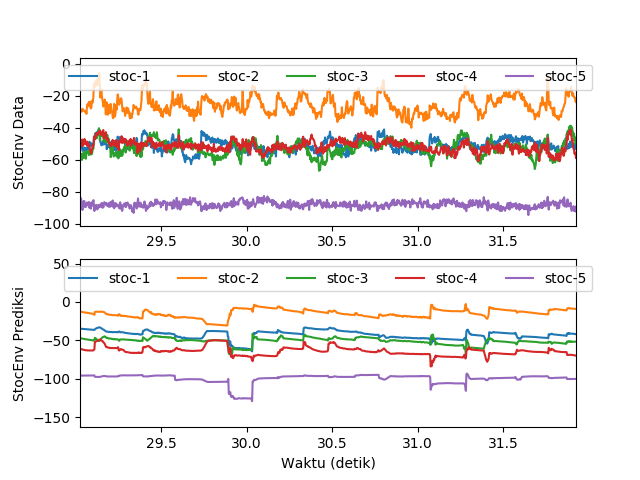
\includegraphics[width=0.8\textwidth]{resources/Analisis_StocEnv_zoomed.png}
    \caption{(Diperbesar) Contoh Keluaran Model Amplop Stokastik, dengan Masukan \textit{Timing}, F0, dan Hfreq dari Dataset}\label{fig-stocenv-output-sample-zoomed}
\end{figure}

Kekurangan yang masih terjadi di model amplop stokastik adalah menganggap perubahan jangka-pendek dari amplop stokastik sebagai \textit{noise} dan hanya dirata-ratakan oleh model. Hal ini tampak pada contoh keluaran model amplop stokastik pada Gambar \ref{fig-stocenv-output-sample}. Pada bagian atas terlihat contoh amplop stokastik dari dataset, sedangkan pada bagian bawah terlihat amplop stokastik prediksi untuk sampel tersebut. Tampilan yang diperbesar tampak pada gambar \ref{fig-stocenv-output-sample-zoomed}.

Terdapat perbedaan antara amplop stokastik data dan amplop stokastik bangkitan:

\begin{itemize}
	\item Amplop stokastik data memiliki naik-turun dan \textit{spike} yang lebih besar
	\item Pada beberapa bagian, perubahan amplop stokastik bangkitan terbalik apabila dibandingkan dengan data
\end{itemize}

Amplop stokastik bangkitan memiliki naik-turun dan \textit{spike} yang kurang besar karena sebagian besar naik turun dan \textit{spike} tersebut dianggap sebagai \textit{noise} oleh model. Jaringan syaraf tiruan yang digunakan kemudian merata-ratakannya dan merepresentasikan perubahannya dalam keluaran variansi CGM, yang kemudian dikurangi dengan parameter temperatur.

Pada beberapa bagian, perubahan amplop stokastik bangkitan terbalik apabila dibandingkan dengan data. Di sebagian tempat, besaran amplop stokastik bangkitan turun padahal amplop stokastik pada data naik. Begitu pula sebaliknya, amplop stokastik bangkitan naik padahal amplop stokastik pada data turun. %TODO kenapa? kapan ia terbalik?

%TODO perbandingan hasil,
%TODO pola-pola yang tidak tertangkap oleh koefisien korelasi
%bahwa RPM mungkin saja memiliki nilai lebih tinggi dalam uji persepsi kealamian

\section{Hasil Uji Korelasi Sistem Utuh}
Tabel \ref{tab-system-testing-results} menunjukkan hasil uji korelasi sistem DT-Neural Parametrik dan perbandingannya dengan sistem \textit{baseline} yaitu RPM. Sistem DT-Neural Parametrik berhasil mencapai koefisien korelasi di atas nol, yang artinya sistem ini berhasil mempelajari sebagian pola-pola ekspresi. Namun, nilai koefisien korelasi ini masih rendah, artinya tidak semua pola-pola ekspresi berhasil dipelajari dengan benar.

\begin{table}[htbp]
    \centering
    \caption{Hasil Pengujian Korelasi Sistem Utuh}\label{tab-system-testing-results}
    \begin{tabular}{ |l|r|r| } 
     \cline{2-3}
     \multicolumn{1}{l|}{}&\multicolumn{2}{|l|}{Rata-Rata Pearson r Semua Komponen}\\\hline
     Sistem&Terhadap data latih&Terhadap data uji\\\hline
	 RPM&-0.2380* &-0.0020\\\hline
	 DT-Neural Parametrik& 0.1188**&0.1133\\\hline
	 \multicolumn{3}{l}{*RPM tidak dilatih dengan data latih ini}\\
	 \multicolumn{3}{l}{**Model komponen dilatih dengan subset yang telah dipilih}\\
    \end{tabular}
\end{table}

Nilai koefisien korelasi yang dicapai oleh sistem ini lebih tinggi daripada sistem RPM. Sistem yang diajukan menghasilkan keluaran dengan koefisien korelasi 0.1188 terhadap data latih, sementara RPM hanya menghasilkan -0.2380, dengan catatan bahwa sistem RPM memang tidak dilatih menggunakan data latih ini. Untuk membandingkan kinerja generalisasi kedua sistem, dibandingkan kinerjanya terhadap data uji. Sistem yang diajukan menghasilkan koefisien korelasi 0.1133 terhadap data uji, sementara sistem RPM hanya menghasilkan koefisien  korelasi -0.0020.



%TODO analisis, contoh perbandingan output RPM dan DT-Neural Parametrik

\section{Hasil Uji Preferensi}
\blindtext